% Options for packages loaded elsewhere
\PassOptionsToPackage{unicode}{hyperref}
\PassOptionsToPackage{hyphens}{url}
%
\documentclass[
]{article}
\usepackage{amsmath,amssymb}
\usepackage{lmodern}
\usepackage{ifxetex,ifluatex}
\ifnum 0\ifxetex 1\fi\ifluatex 1\fi=0 % if pdftex
  \usepackage[T1]{fontenc}
  \usepackage[utf8]{inputenc}
  \usepackage{textcomp} % provide euro and other symbols
\else % if luatex or xetex
  \usepackage{unicode-math}
  \defaultfontfeatures{Scale=MatchLowercase}
  \defaultfontfeatures[\rmfamily]{Ligatures=TeX,Scale=1}
\fi
% Use upquote if available, for straight quotes in verbatim environments
\IfFileExists{upquote.sty}{\usepackage{upquote}}{}
\IfFileExists{microtype.sty}{% use microtype if available
  \usepackage[]{microtype}
  \UseMicrotypeSet[protrusion]{basicmath} % disable protrusion for tt fonts
}{}
\makeatletter
\@ifundefined{KOMAClassName}{% if non-KOMA class
  \IfFileExists{parskip.sty}{%
    \usepackage{parskip}
  }{% else
    \setlength{\parindent}{0pt}
    \setlength{\parskip}{6pt plus 2pt minus 1pt}}
}{% if KOMA class
  \KOMAoptions{parskip=half}}
\makeatother
\usepackage{xcolor}
\IfFileExists{xurl.sty}{\usepackage{xurl}}{} % add URL line breaks if available
\IfFileExists{bookmark.sty}{\usepackage{bookmark}}{\usepackage{hyperref}}
\hypersetup{
  pdftitle={R Markdown Guide},
  hidelinks,
  pdfcreator={LaTeX via pandoc}}
\urlstyle{same} % disable monospaced font for URLs
\usepackage[margin=1in]{geometry}
\usepackage{color}
\usepackage{fancyvrb}
\newcommand{\VerbBar}{|}
\newcommand{\VERB}{\Verb[commandchars=\\\{\}]}
\DefineVerbatimEnvironment{Highlighting}{Verbatim}{commandchars=\\\{\}}
% Add ',fontsize=\small' for more characters per line
\usepackage{framed}
\definecolor{shadecolor}{RGB}{248,248,248}
\newenvironment{Shaded}{\begin{snugshade}}{\end{snugshade}}
\newcommand{\AlertTok}[1]{\textcolor[rgb]{0.94,0.16,0.16}{#1}}
\newcommand{\AnnotationTok}[1]{\textcolor[rgb]{0.56,0.35,0.01}{\textbf{\textit{#1}}}}
\newcommand{\AttributeTok}[1]{\textcolor[rgb]{0.77,0.63,0.00}{#1}}
\newcommand{\BaseNTok}[1]{\textcolor[rgb]{0.00,0.00,0.81}{#1}}
\newcommand{\BuiltInTok}[1]{#1}
\newcommand{\CharTok}[1]{\textcolor[rgb]{0.31,0.60,0.02}{#1}}
\newcommand{\CommentTok}[1]{\textcolor[rgb]{0.56,0.35,0.01}{\textit{#1}}}
\newcommand{\CommentVarTok}[1]{\textcolor[rgb]{0.56,0.35,0.01}{\textbf{\textit{#1}}}}
\newcommand{\ConstantTok}[1]{\textcolor[rgb]{0.00,0.00,0.00}{#1}}
\newcommand{\ControlFlowTok}[1]{\textcolor[rgb]{0.13,0.29,0.53}{\textbf{#1}}}
\newcommand{\DataTypeTok}[1]{\textcolor[rgb]{0.13,0.29,0.53}{#1}}
\newcommand{\DecValTok}[1]{\textcolor[rgb]{0.00,0.00,0.81}{#1}}
\newcommand{\DocumentationTok}[1]{\textcolor[rgb]{0.56,0.35,0.01}{\textbf{\textit{#1}}}}
\newcommand{\ErrorTok}[1]{\textcolor[rgb]{0.64,0.00,0.00}{\textbf{#1}}}
\newcommand{\ExtensionTok}[1]{#1}
\newcommand{\FloatTok}[1]{\textcolor[rgb]{0.00,0.00,0.81}{#1}}
\newcommand{\FunctionTok}[1]{\textcolor[rgb]{0.00,0.00,0.00}{#1}}
\newcommand{\ImportTok}[1]{#1}
\newcommand{\InformationTok}[1]{\textcolor[rgb]{0.56,0.35,0.01}{\textbf{\textit{#1}}}}
\newcommand{\KeywordTok}[1]{\textcolor[rgb]{0.13,0.29,0.53}{\textbf{#1}}}
\newcommand{\NormalTok}[1]{#1}
\newcommand{\OperatorTok}[1]{\textcolor[rgb]{0.81,0.36,0.00}{\textbf{#1}}}
\newcommand{\OtherTok}[1]{\textcolor[rgb]{0.56,0.35,0.01}{#1}}
\newcommand{\PreprocessorTok}[1]{\textcolor[rgb]{0.56,0.35,0.01}{\textit{#1}}}
\newcommand{\RegionMarkerTok}[1]{#1}
\newcommand{\SpecialCharTok}[1]{\textcolor[rgb]{0.00,0.00,0.00}{#1}}
\newcommand{\SpecialStringTok}[1]{\textcolor[rgb]{0.31,0.60,0.02}{#1}}
\newcommand{\StringTok}[1]{\textcolor[rgb]{0.31,0.60,0.02}{#1}}
\newcommand{\VariableTok}[1]{\textcolor[rgb]{0.00,0.00,0.00}{#1}}
\newcommand{\VerbatimStringTok}[1]{\textcolor[rgb]{0.31,0.60,0.02}{#1}}
\newcommand{\WarningTok}[1]{\textcolor[rgb]{0.56,0.35,0.01}{\textbf{\textit{#1}}}}
\usepackage{graphicx}
\makeatletter
\def\maxwidth{\ifdim\Gin@nat@width>\linewidth\linewidth\else\Gin@nat@width\fi}
\def\maxheight{\ifdim\Gin@nat@height>\textheight\textheight\else\Gin@nat@height\fi}
\makeatother
% Scale images if necessary, so that they will not overflow the page
% margins by default, and it is still possible to overwrite the defaults
% using explicit options in \includegraphics[width, height, ...]{}
\setkeys{Gin}{width=\maxwidth,height=\maxheight,keepaspectratio}
% Set default figure placement to htbp
\makeatletter
\def\fps@figure{htbp}
\makeatother
\setlength{\emergencystretch}{3em} % prevent overfull lines
\providecommand{\tightlist}{%
  \setlength{\itemsep}{0pt}\setlength{\parskip}{0pt}}
\setcounter{secnumdepth}{-\maxdimen} % remove section numbering
\usepackage[labelfont=bf, margin=2in]{caption}
\usepackage{floatrow}
\floatsetup[table]{capposition=top}
\ifluatex
  \usepackage{selnolig}  % disable illegal ligatures
\fi

\title{R Markdown Guide}
\author{}
\date{\vspace{-2.5em}}

\begin{document}
\maketitle

Files with the extension .rmd are known as R markdown files. These files
combine the use of markdown, which can convert text into many different
formats (html, pdf, Microsoft word, etc.), with the use of R code. This
allows you to create documents with pretty text and data analysis all in
one. This file will knit without errors and is a resource for you to see
how what is written in a .rmd translates when it is knit to a pdf.

In this document the white space contains markdown text while the gray
boxes contain R code. In markdown text, spaces between words actually
produce spaces. Here are some other examples of how to format your
document.

\#\#Example: Starting a New Paragraph

I want this to be in paragraph 1. I want this to be in paragraph 2.

vs

I want this to be in paragraph 1.

I want this to be in paragraph 2.

\textbf{By putting two line spaces in between text you can break the
line.}

\#\#Example: Bold and Italic Text

This is normal text

\textbf{This is bold text}

\emph{This is italicized text}

\#\#Example: Making Headers

\#Header size 1

\#\#Header size 2

\#\#\#Header size 3

\#\#\#\#Header size 4

\#\#How to Add Links

In {[}{]} add the name for the link and in () add the URL for the link

\href{https://www.codecogs.com/latex/eqneditor.php}{Latex Equation
Editor}

\#\#Example: How to Make Pretty Equations!

We can use Latex code in a markdown file to format equations by putting
it in between two \$ signs

For an in line equation we can use \(y = mx + b\)

For an stand alone equation we want to be centered on the page we can
use \[ y = mx + b \]

\textbf{Here are some common examples of equations you will use in
chemistry.}

Beer's law is \(A = a b c\) where A is the absorbance, \(a\) is the
molar absorbtivity in units of \(M^{-1} cm^{-1}\) \(b\) is the path
length in \(cm\), and \(c\) is the concentration in \(M\).

\textbf{Conversions}

\(P_{atm} = 29.83\: in\: Hg\: * \frac{2.54\: cm}{1\: in} * \frac{1000\: mm}{1\: cm} * \frac{1\: atm}{760\: mm\: Hg}\)

In equations to add spaces, \(29.83 in Hg\) must be written as
\(29.83\: in \: Hg\).

\textbf{Supercript and Subscript}

\(P_{atm}\) vs \(P^{atm}\), the sub-scripted or super-scripted text must
be written within the \{\}

\(1.3 \times 10^{-3}\)

\(S_{2}O_{8}^{2-}\)

\textbf{Fractions}

\(\frac{a}{b}\) \(\frac{1}{1000}\)

You can also do sub scripts and super scripts within fractions\ldots{}

\(K_{a} = \frac{[A^{-}][H_{3}O^{+}]}{[HA]}\)

\textbf{Commonly Used Symbols}

Degree Symbol: \(^\circ\), e.g.~25 \(^\circ\)C

Delta Symbol: \(\Delta\), e.g.~\(\Delta{A}\)

Less Than/Greater Than: \textless{} / \textgreater{} , e.g.~10
\textless{} 30

Plus or Minus Sign: \(\pm\), e.g.~5.0 \(\pm\) 0.2

Percent Sign: \%, e.g.~25 \%

\textbf{More Example Equations}

\(P = \frac{nRT}{V}\)

\(x = \sqrt{x^{2}}\)

\(rate = k[I^{-}]^{m}\,[S_{2}O_{8}^{2-}]^{n}\)

Arrhenius Equation

\(k = Ae^{-E_{a}/RT}\)

\clearpage

This pushes everything after it to the next page

\textbf{If you want to get fancy\ldots you can also write reaction
equations}

Mechanism A:

\(S_{2}O_{8}^{2-} \rightarrow SO_{4} + SO_{4}^{2-} \: (slow)\)

\(SO_{4} + I^{-} \rightarrow SO_{4}^{2-} + I^{+}\)

\(I^{+} + I^{-} \rightarrow I_{2}\)

\(I_{2} + I^{-} \rightarrow I_{3}^{-}\)

\textbf{Reactions in Equilibrium}

\(X_{(l)} \rightleftharpoons X_{(g)}\)

\(2H_{2}O_{l} \rightleftharpoons H_{3}O^{+}_{aq} + OH^{-}_{aq}\)

\#\#Example: Adding Images

\texttt{!{[}Caption\ of\ Photo{]}(name\ of\ file)}

Follow this format without the \texttt{} and make sure the image is in
the same folder as your .rmd file to which you are trying to add the
image.

\#\#Now for some R code Examples

R code is written in gray chunks, which start with
\texttt{\{r\}\ and\ end\ with} (see below)

Comments can be added to the code by adding a \# in front of text

\begin{Shaded}
\begin{Highlighting}[]
\NormalTok{x }\OtherTok{\textless{}{-}} \DecValTok{10} \SpecialCharTok{+} \DecValTok{5} \CommentTok{\# x is the number 15}

\FunctionTok{print}\NormalTok{(x) }\CommentTok{\#this function prints what x is}
\end{Highlighting}
\end{Shaded}

\begin{verbatim}
## [1] 15
\end{verbatim}

\begin{Shaded}
\begin{Highlighting}[]
\NormalTok{x }\OtherTok{\textless{}{-}} \FunctionTok{as.numeric}\NormalTok{(}\FunctionTok{c}\NormalTok{(}\StringTok{"1"}\NormalTok{, }\StringTok{"2"}\NormalTok{, }\StringTok{"X"}\NormalTok{)) }\CommentTok{\# Code that gives a warning. It converts X to NA and is warning that this is what is happening}
\end{Highlighting}
\end{Shaded}

\begin{verbatim}
## Warning: NAs introduced by coercion
\end{verbatim}

\begin{Shaded}
\begin{Highlighting}[]
\NormalTok{pkg }\OtherTok{\textless{}{-}} \FunctionTok{c}\NormalTok{(}\StringTok{"dplyr"}\NormalTok{, }\StringTok{"knitr"}\NormalTok{, }\StringTok{"xtable"}\NormalTok{, }\StringTok{"rmarkdown"}\NormalTok{, }\StringTok{"readr"}\NormalTok{, }\StringTok{"ggplot2"}\NormalTok{)}

\NormalTok{new.pkg }\OtherTok{\textless{}{-}}\NormalTok{ pkg[}\SpecialCharTok{!}\NormalTok{(pkg }\SpecialCharTok{\%in\%} \FunctionTok{installed.packages}\NormalTok{())]}

\ControlFlowTok{if}\NormalTok{ (}\FunctionTok{length}\NormalTok{(new.pkg)) \{}

  \FunctionTok{install.packages}\NormalTok{(new.pkg, }\AttributeTok{repos =} \StringTok{"http://cran.rstudio.com"}\NormalTok{)}
  
\NormalTok{\}}

\FunctionTok{library}\NormalTok{(dplyr) }\CommentTok{\# Code that produces messages}
\end{Highlighting}
\end{Shaded}

\begin{verbatim}
## 
## Attaching package: 'dplyr'
\end{verbatim}

\begin{verbatim}
## The following objects are masked from 'package:stats':
## 
##     filter, lag
\end{verbatim}

\begin{verbatim}
## The following objects are masked from 'package:base':
## 
##     intersect, setdiff, setequal, union
\end{verbatim}

\begin{Shaded}
\begin{Highlighting}[]
\FunctionTok{library}\NormalTok{(xtable)}
\end{Highlighting}
\end{Shaded}

We can choose not to show messages from the code in the pdf by adding
messages = FALSE to the beginning of the chunk ```\{r, message = FALSE\}
(see below)

\begin{Shaded}
\begin{Highlighting}[]
\NormalTok{x }\OtherTok{\textless{}{-}} \DecValTok{10} \SpecialCharTok{+} \DecValTok{5} \CommentTok{\# x is the number 15}

\FunctionTok{print}\NormalTok{(x) }\CommentTok{\#this function prints what x is}
\end{Highlighting}
\end{Shaded}

\begin{verbatim}
## [1] 15
\end{verbatim}

\begin{Shaded}
\begin{Highlighting}[]
\NormalTok{x }\OtherTok{\textless{}{-}} \FunctionTok{as.numeric}\NormalTok{(}\FunctionTok{c}\NormalTok{(}\StringTok{"1"}\NormalTok{, }\StringTok{"2"}\NormalTok{, }\StringTok{"X"}\NormalTok{)) }\CommentTok{\# Code that gives a warning. It converts X to NA and is warning that this is what is happening}
\end{Highlighting}
\end{Shaded}

\begin{verbatim}
## Warning: NAs introduced by coercion
\end{verbatim}

\begin{Shaded}
\begin{Highlighting}[]
\NormalTok{pkg }\OtherTok{\textless{}{-}} \FunctionTok{c}\NormalTok{(}\StringTok{"dplyr"}\NormalTok{, }\StringTok{"knitr"}\NormalTok{, }\StringTok{"xtable"}\NormalTok{, }\StringTok{"rmarkdown"}\NormalTok{, }\StringTok{"readr"}\NormalTok{, }\StringTok{"ggplot2"}\NormalTok{)}

\NormalTok{new.pkg }\OtherTok{\textless{}{-}}\NormalTok{ pkg[}\SpecialCharTok{!}\NormalTok{(pkg }\SpecialCharTok{\%in\%} \FunctionTok{installed.packages}\NormalTok{())]}

\ControlFlowTok{if}\NormalTok{ (}\FunctionTok{length}\NormalTok{(new.pkg)) \{}

  \FunctionTok{install.packages}\NormalTok{(new.pkg, }\AttributeTok{repos =} \StringTok{"http://cran.rstudio.com"}\NormalTok{)}
  
\NormalTok{\}}

\FunctionTok{library}\NormalTok{(dplyr) }\CommentTok{\# Code that produces messages}
\end{Highlighting}
\end{Shaded}

We can control whether or not the code is shown in the pdf by adding
echo = FALSE to the beginning of the chunk ```\{r, echo = FALSE\} (see
below)

\begin{verbatim}
## [1] 15
\end{verbatim}

\begin{verbatim}
## Warning: NAs introduced by coercion
\end{verbatim}

We can choose not to show warnings from the code in the pdf by adding
warning = FALSE to the beginning of the chunk ```\{r, warning = FALSE\}
(see below)

\begin{verbatim}
## [1] 15
\end{verbatim}

\clearpage

The \% symbol in LaTex is used for comments. When writing r code (only
gray chunks) either avoid using the percent symbol (in captions for
tables and such) or use \textbackslash\%. If when trying to knit to pdf
you get an error message in red that reads, ! File ended while scanning
use of \textbf, then you have used the percent symbol somewhere in the
file where it is being read as a comment in LaTex. To fix the error, try
either removing \% symbols from r code or using \textbackslash\%.

\hypertarget{example-creating-plots-in-r}{%
\subsection{Example: Creating Plots in
R}\label{example-creating-plots-in-r}}

\begin{Shaded}
\begin{Highlighting}[]
\CommentTok{\# Add caption title within quotes above }

\CommentTok{\#Defining values for x and y to plot}
\NormalTok{x }\OtherTok{\textless{}{-}} \FunctionTok{c}\NormalTok{(}\DecValTok{1}\NormalTok{, }\FloatTok{2.2}\NormalTok{, }\DecValTok{4}\NormalTok{, }\FloatTok{6.3}\NormalTok{, }\FloatTok{8.1}\NormalTok{) }
\NormalTok{y }\OtherTok{\textless{}{-}} \FunctionTok{c}\NormalTok{(}\DecValTok{5}\NormalTok{, }\FloatTok{7.2}\NormalTok{, }\FloatTok{8.4}\NormalTok{, }\FloatTok{9.5}\NormalTok{, }\FloatTok{12.3}\NormalTok{)}

\CommentTok{\#Basic plot of y vs x (2 options)}

\FunctionTok{plot}\NormalTok{(x, y)}
\end{Highlighting}
\end{Shaded}

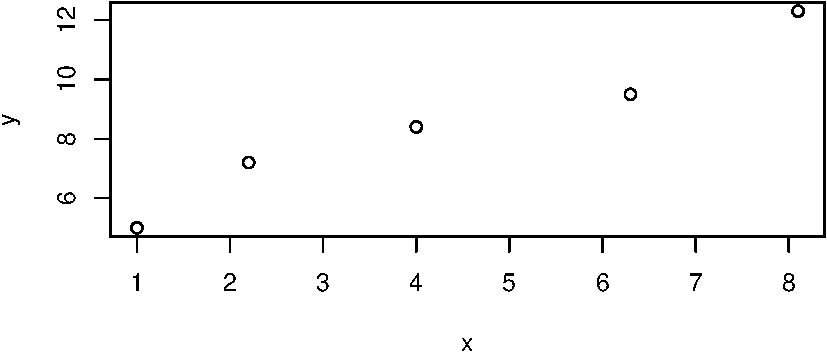
\includegraphics{skeleton_files/figure-latex/unnamed-chunk-5-1.pdf}

\begin{Shaded}
\begin{Highlighting}[]
\CommentTok{\#or}

\FunctionTok{plot}\NormalTok{(y }\SpecialCharTok{\textasciitilde{}}\NormalTok{ x)}
\end{Highlighting}
\end{Shaded}

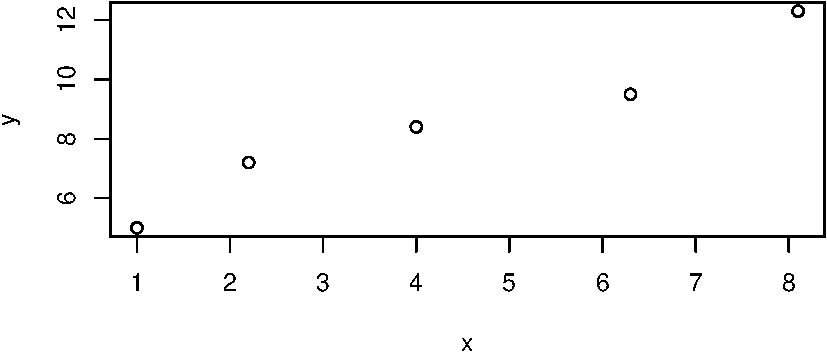
\includegraphics{skeleton_files/figure-latex/unnamed-chunk-5-2.pdf}

\begin{Shaded}
\begin{Highlighting}[]
\CommentTok{\# The data look pretty linear, so let\textquotesingle{}s fit a straight line (y = mx + b) to it }
\CommentTok{\# and plot with the best fit line}

\CommentTok{\# First, let\textquotesingle{}s put x and y values into a dataframe, much like columns in excel}
\NormalTok{x.and.y }\OtherTok{\textless{}{-}} \FunctionTok{data\_frame}\NormalTok{(x, y) }
\end{Highlighting}
\end{Shaded}

\begin{verbatim}
## Warning: `data_frame()` was deprecated in tibble 1.1.0.
## Please use `tibble()` instead.
## This warning is displayed once every 8 hours.
## Call `lifecycle::last_lifecycle_warnings()` to see where this warning was generated.
\end{verbatim}

\begin{Shaded}
\begin{Highlighting}[]
\CommentTok{\# Take a look at the data frame by typing the name for the data frame}
\NormalTok{x.and.y}
\end{Highlighting}
\end{Shaded}

\begin{verbatim}
## # A tibble: 5 x 2
##       x     y
##   <dbl> <dbl>
## 1   1     5  
## 2   2.2   7.2
## 3   4     8.4
## 4   6.3   9.5
## 5   8.1  12.3
\end{verbatim}

\begin{Shaded}
\begin{Highlighting}[]
\CommentTok{\# Let\textquotesingle{}s fit the data to our equation y = mx + b}
\NormalTok{fit }\OtherTok{\textless{}{-}} \FunctionTok{nls}\NormalTok{(y }\SpecialCharTok{\textasciitilde{}}\NormalTok{ m}\SpecialCharTok{*}\NormalTok{x }\SpecialCharTok{+}\NormalTok{ b, }\AttributeTok{data =}\NormalTok{ x.and.y, }\AttributeTok{start =} \FunctionTok{list}\NormalTok{(}\AttributeTok{m =} \DecValTok{1}\NormalTok{, }\AttributeTok{b =} \DecValTok{4}\NormalTok{)) }\CommentTok{\# put in }
\CommentTok{\# very rough guesses for slope (m) and y intercept (b)}

\CommentTok{\# Now for every x value we have we want the y values that the equation }
\CommentTok{\# predicts in order to plot the best fit line. We can extract these as a }
\CommentTok{\# vector by using the function as.vector() and the function fitted().}
\NormalTok{ycalc }\OtherTok{\textless{}{-}} \FunctionTok{as.vector}\NormalTok{(}\FunctionTok{fitted}\NormalTok{(fit))}

\CommentTok{\# Now let\textquotesingle{}s plot our data with the best fit line using the function lines()}
\FunctionTok{plot}\NormalTok{(x, y)}
\FunctionTok{lines}\NormalTok{(x, ycalc)}
\end{Highlighting}
\end{Shaded}

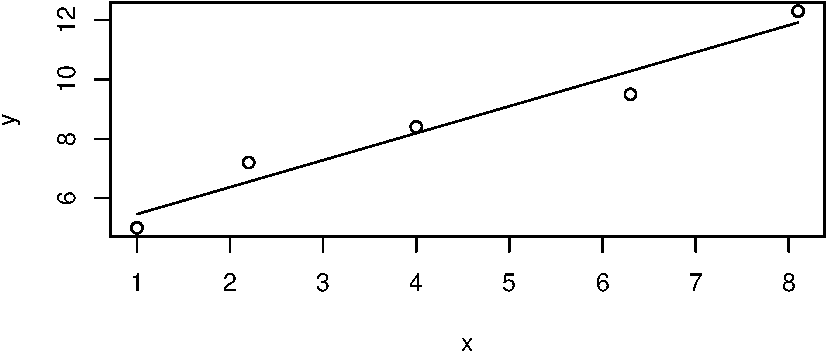
\includegraphics{skeleton_files/figure-latex/unnamed-chunk-5-3.pdf}

\begin{Shaded}
\begin{Highlighting}[]
\CommentTok{\# To produce a plot with colored lines and solid black dots use this}
\FunctionTok{plot}\NormalTok{(x, y,}
     \AttributeTok{pch =} \DecValTok{20}\NormalTok{)}
\FunctionTok{lines}\NormalTok{(x, ycalc, }\AttributeTok{col =} \StringTok{"blue"}\NormalTok{)}
\end{Highlighting}
\end{Shaded}

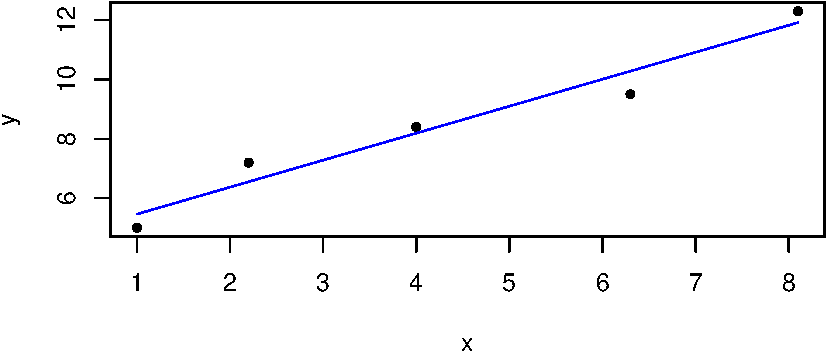
\includegraphics{skeleton_files/figure-latex/unnamed-chunk-5-4.pdf}

\textbf{Adding Axis Labels and Captions with Superscripts and
Subscripts)}

Now let's reassign x to be concentration of persulfate and y to be rate
when varying persulfate concentration

\begin{Shaded}
\begin{Highlighting}[]
\CommentTok{\# Add caption title within quotes above }

\CommentTok{\# reassigning x and y }
\NormalTok{rate }\OtherTok{\textless{}{-}}\NormalTok{ y}
\NormalTok{persulfate.conc }\OtherTok{\textless{}{-}}\NormalTok{ x}
\NormalTok{fitted.rate }\OtherTok{\textless{}{-}}\NormalTok{ ycalc}

\CommentTok{\# Plot of rate vs persulfate concentration with appropriate labels that include units}
\CommentTok{\# Within expression function, \textasciitilde{} is for a space while * is for no space, [] is for }
\CommentTok{\# subscript, \^{} is for superscript }

\FunctionTok{plot}\NormalTok{(persulfate.conc, rate,}
    \AttributeTok{xlab =} \FunctionTok{expression}\NormalTok{(}\StringTok{"["} \SpecialCharTok{\textasciitilde{}}\NormalTok{ S[}\DecValTok{2}\NormalTok{] }\SpecialCharTok{*}\NormalTok{ O[}\DecValTok{8}\NormalTok{]}\SpecialCharTok{\^{}}\StringTok{"2{-}"} \SpecialCharTok{\textasciitilde{}} \StringTok{"]"}  \SpecialCharTok{\textasciitilde{}}\NormalTok{ (M)),   }
    \AttributeTok{ylab =} \FunctionTok{expression}\NormalTok{(}\StringTok{"Rate"} \SpecialCharTok{\textasciitilde{}}\NormalTok{ (}\StringTok{"M"} \SpecialCharTok{*}\NormalTok{ s}\SpecialCharTok{\^{}{-}}\DecValTok{1}\NormalTok{)),}
     \AttributeTok{pch =} \DecValTok{20}\NormalTok{)}
\FunctionTok{lines}\NormalTok{(persulfate.conc, fitted.rate, }\AttributeTok{col =} \StringTok{"green"}\NormalTok{)}
\end{Highlighting}
\end{Shaded}

\begin{figure}
\centering
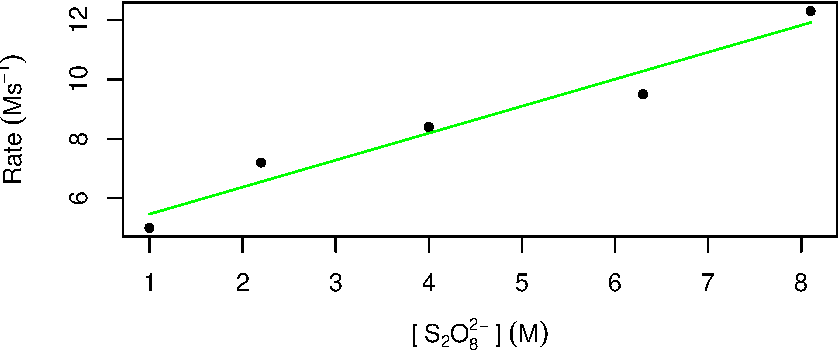
\includegraphics{skeleton_files/figure-latex/unnamed-chunk-6-1.pdf}
\caption{Plot of Rate vs Persulfate Concentration}
\end{figure}

\hypertarget{example-creating-tables}{%
\subsection{Example: Creating Tables}\label{example-creating-tables}}

\begin{table}[ht]
\centering
\parbox{2.7in}{\caption{Rate and Persulfate Concentration}} 
\begin{tabular}{|r|r|}
  \hline
\textbf{Rate (M/s)} & \textbf{Persulfate Concentration (M)} \\ 
  \hline
5.0 & 1.00 \\ 
   \hline
7.2 & 2.20 \\ 
   \hline
8.4 & 4.00 \\ 
   \hline
9.5 & 6.30 \\ 
   \hline
12.3 & 8.10 \\ 
   \hline
\end{tabular}
\end{table}

\end{document}
